\subsection{Surface scattering models}
\begin{figure}[h!]
\centering
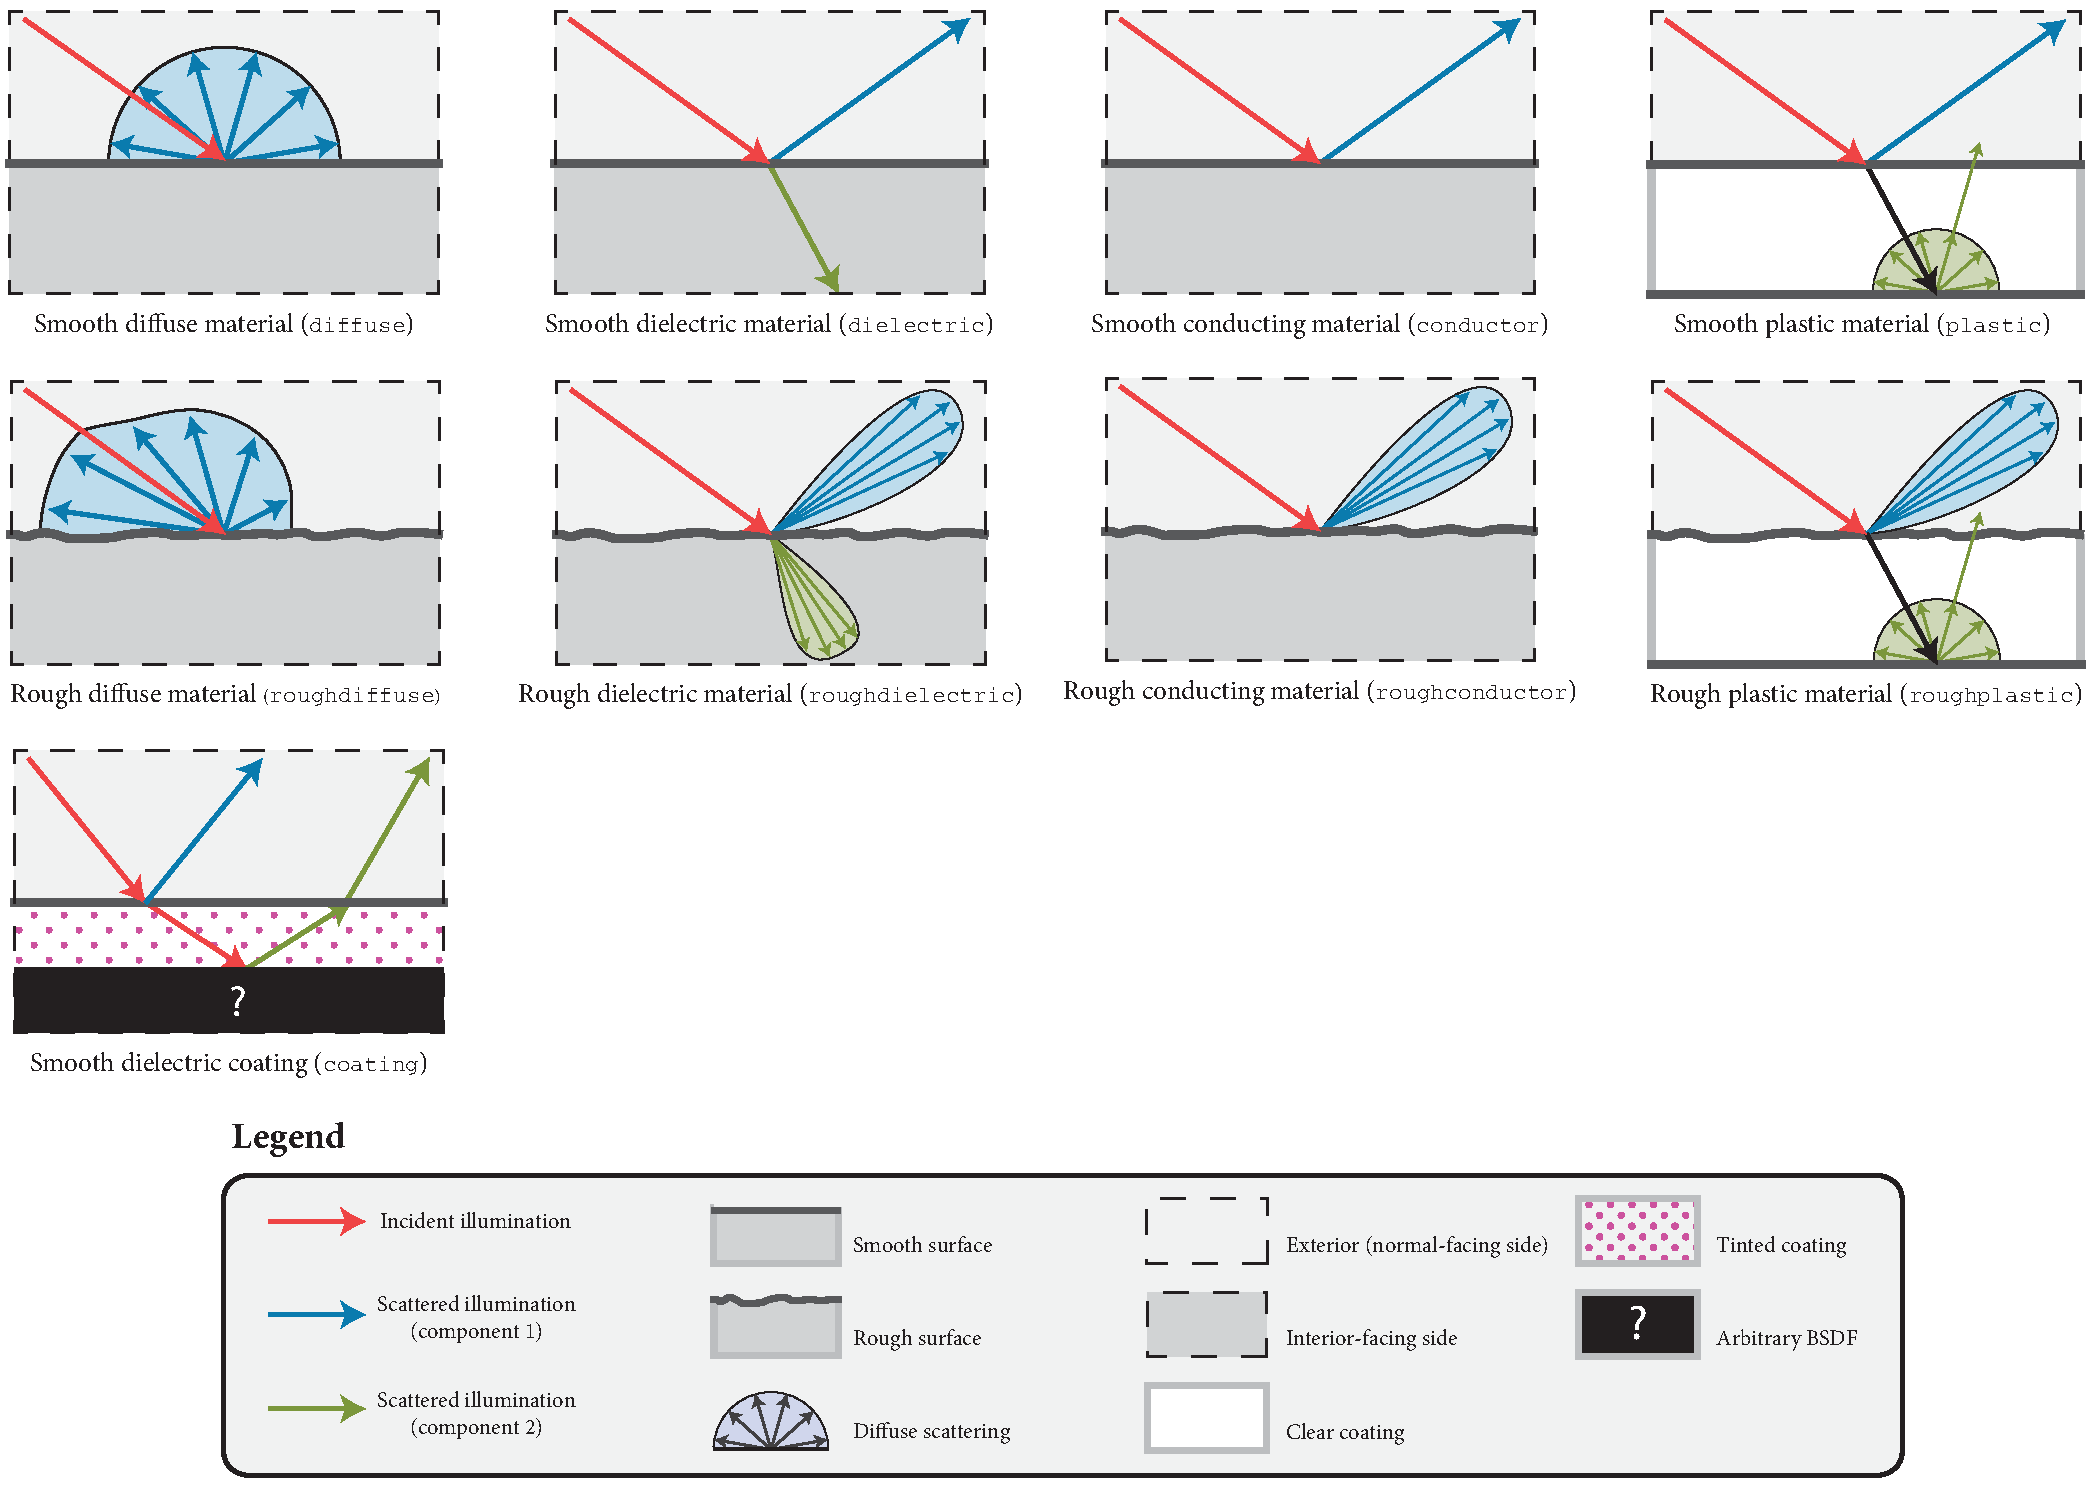
\includegraphics[width=15.5cm]{images/bsdf_overview.pdf}
\caption{
	Schematic overview of the most important surface scattering models in
	Mitsuba (shown in the style of Weidlich and Wilkie \cite{Weidlich2007Arbitrarily}). The arrows indicate possible outcomes of an
	interaction with a surface that has the respective model applied to it.
	\vspace{4mm}
}
\end{figure}

\label{sec:bsdfs}
Surface scattering models describe the manner in which light interacts
with surfaces in the scene. They conveniently summarize the mesoscopic 
scattering processes that take place within the material and 
cause it to look the way it does.
This represents one central component of the material system in Mitsuba---another 
part of the renderer concerns itself with what happens 
\emph{in between} surface interactions. For more information on this aspect, 
please refer to Sections~\ref{sec:media} and \ref{sec:subsurface}.
This section presents an overview of all surface scattering models that are 
supported, along with their parameters.

\subsubsection*{BSDFs}
To achieve realistic results, Mitsuba comes with a library of both 
general-purpose surface scattering models (smooth or rough glass, metal,
plastic, etc.) and specializations to particular materials (woven cloth,
masks, etc.). Some model plugins fit neither category and can best be described
as \emph{modifiers} that are applied on top of one or more scattering models. 

Throughout the documentation and within the scene description 
language,  the word \emph{BSDF} is used synonymously with the term ``surface
scattering model''. This is an abbreviation for \emph{Bidirectional 
Scattering Distribution Function}, a more precise technical 
term. 

In Mitsuba, BSDFs are 
assigned to \emph{shapes}, which describe the visible surfaces in
the scene. In the scene description language, this assignment can
either be performed by nesting BSDFs within shapes, or they can 
be named and then later referenced by their name. 
The following fragment shows an example of both kinds of usages:
\begin{xml}
<scene version=$\MtsVer$>
	<!-- Creating a named BSDF for later use -->
	<bsdf type=".. BSDF type .." id="myNamedMaterial">
		<!-- BSDF parameters go here -->
	</bsdf>

	<shape type="sphere">
		<!-- Example of referencing a named material -->
		<ref id="myNamedMaterial"/>
	</shape>

	<shape type="sphere">
		<!-- Example of instantiating an unnamed material -->
		<bsdf type=".. BSDF type ..">
			<!-- BSDF parameters go here -->
		</bsdf>
	</shape>
</scene>
\end{xml}
It is generally more economical to use named BSDFs when they
are used in several places, since this reduces Mitsuba's internal
memory usage.
\subsubsection*{Correctness considerations}
\begin{figure}[b!]
\centering
\vspace{-5mm}
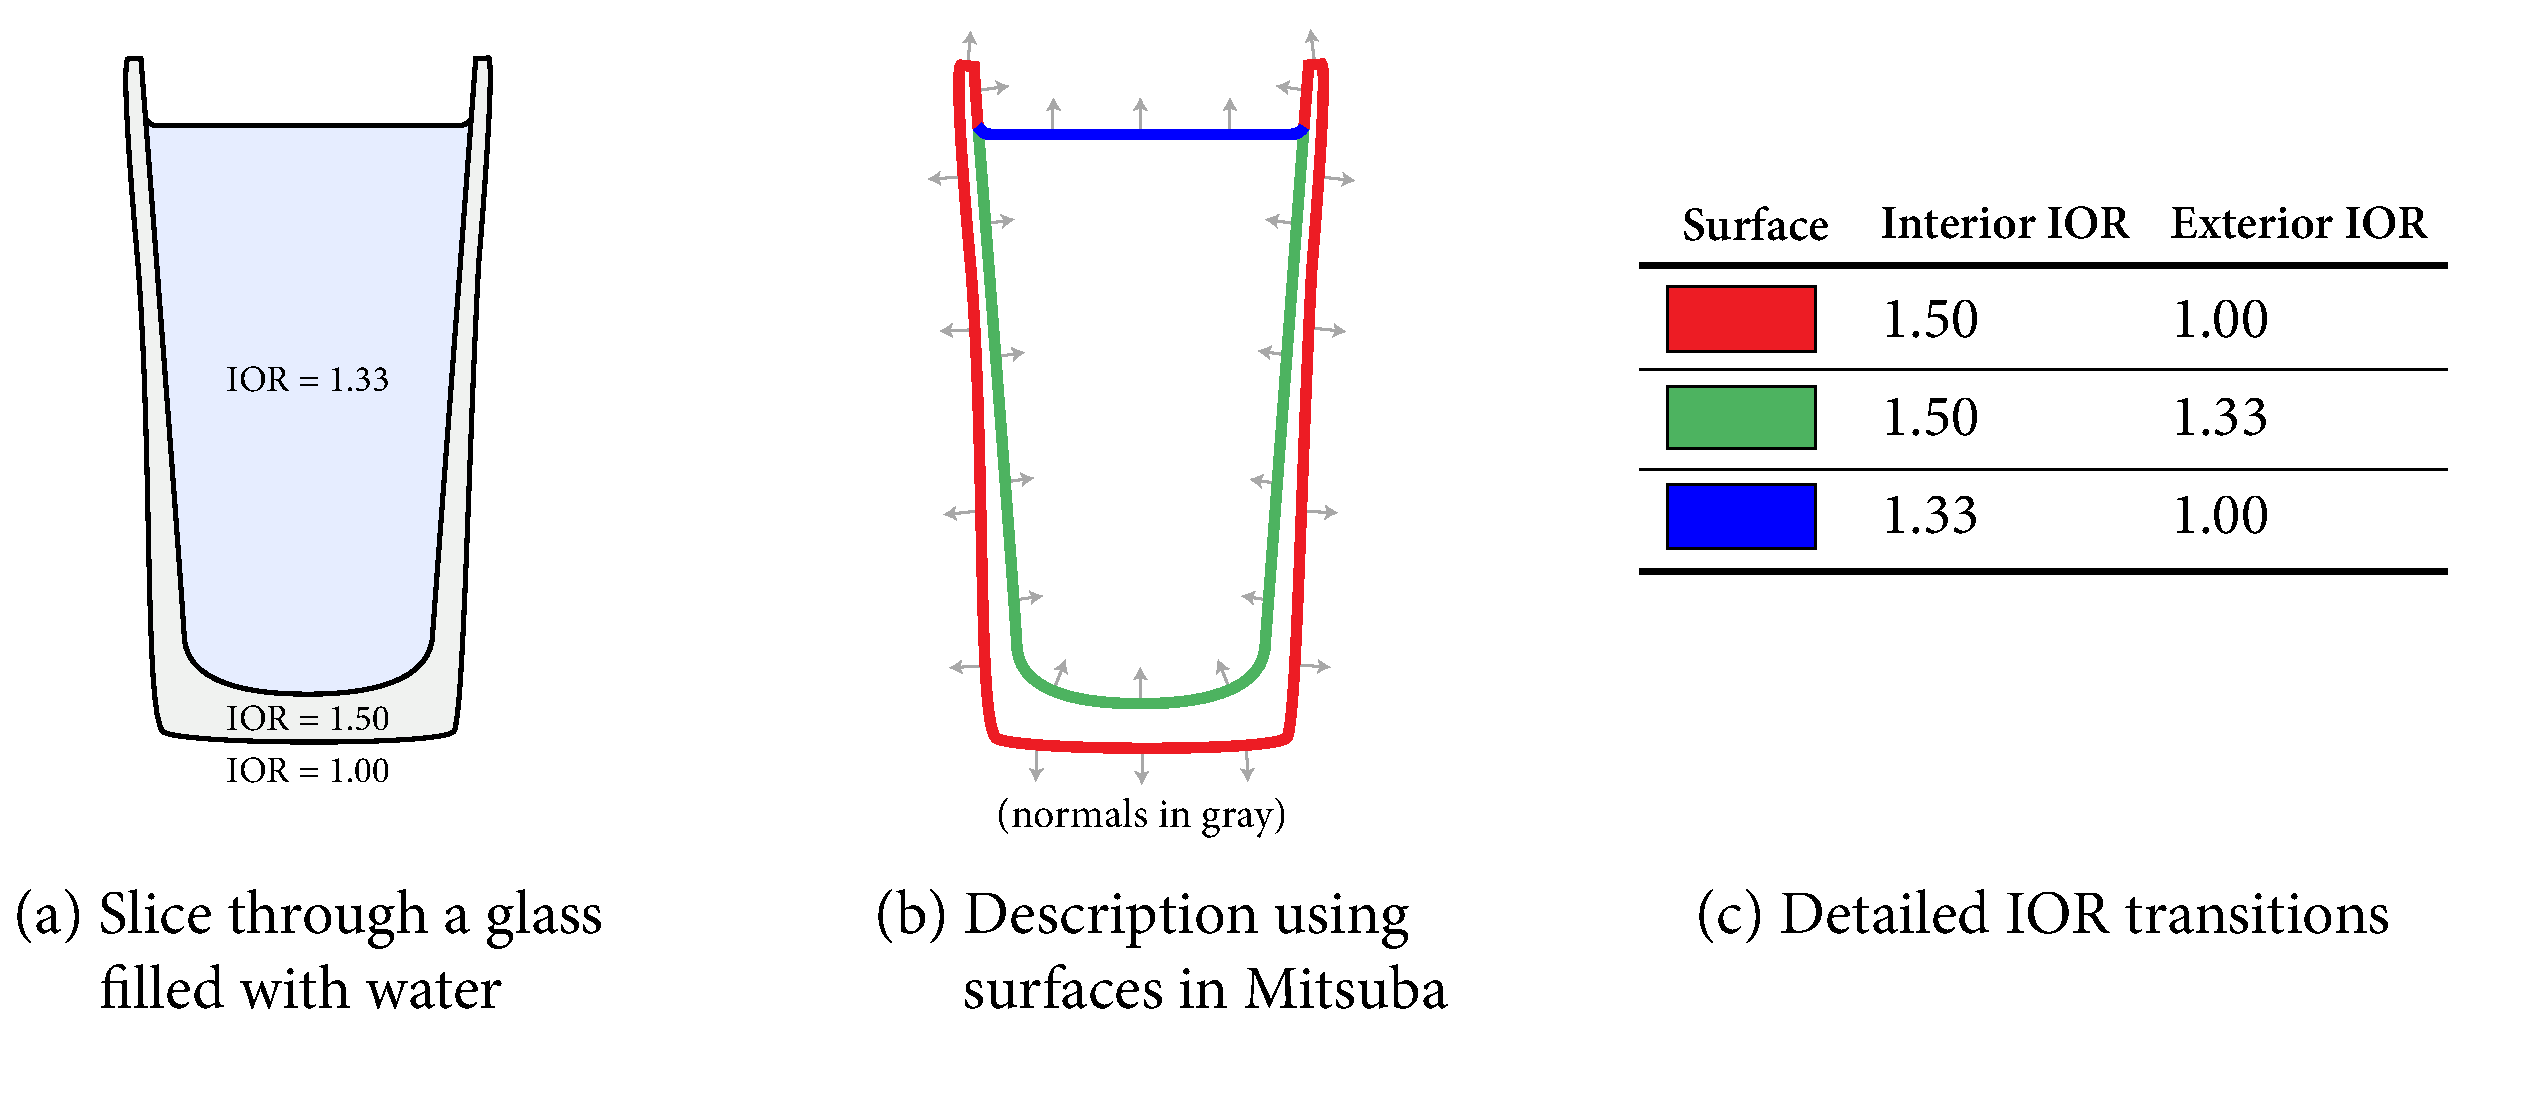
\includegraphics[width=15cm]{images/glass_explanation.pdf}
\vspace{-5mm}
\caption{
	\label{fig:glass-explanation}
	Some of the scattering models in Mitsuba need to know
	the indices of refraction on the exterior and interior-facing
	side of a surface. 
	It is therefore important to decompose the mesh into meaningful
	separate surfaces corresponding to each index of refraction change.
	The example here shows such a decomposition for a water-filled Glass.
}
\end{figure}

A vital consideration when modeling a scene in a physically-based rendering 
system is that the used materials do not violate physical properties, and 
that their arrangement is meaningful. For instance, imagine having designed
an architectural interior scene that looks good except for a white desk that 
seems a bit too dark. A closer inspection reveals that it uses a Lambertian 
material with a diffuse reflectance of $0.9$. 

In many rendering systems, it would be feasible to increase the 
reflectance value above $1.0$ in such a situation. But in Mitsuba, even a 
small surface that reflects a little more light than it receives will 
likely break the available rendering algorithms, or cause them to produce otherwise 
unpredictable results. In fact, we should rather change the lighting setup and
then \emph{reduce} the material's reflectance, since it is quite unlikely that 
we could find a real-world desk with a reflectance as high as $0.9$.

As an example of the necessity for a meaningful material arrangement, consider
the glass model illustrated in \figref{glass-explanation}. Here, careful thinking 
is needed to decompose the object into boundaries that mark index of 
refraction-changes. If this is done incorrectly and a beam of light can
potentially pass through a sequence of incompatible index of refraction changes (e.g. $1.00\to 1.33$
followed by $1.50\to1.33$), the output is undefined and will quite likely
even contain inaccuracies in parts of the scene that are some distance
away from the glass.


